\documentclass[10pt,twocolumn,letterpaper]{article}

\usepackage{cvpr}
\usepackage{times}
\usepackage{epsfig}
\usepackage{graphicx}
\usepackage{amsmath}
\usepackage{amssymb}

% Include other packages here, before hyperref.

% If you comment hyperref and then uncomment it, you should delete
% egpaper.aux before re-running latex.  (Or just hit 'q' on the first latex
% run, let it finish, and you should be clear).
\usepackage[breaklinks=true,bookmarks=false]{hyperref}

\cvprfinalcopy{} % *** Uncomment this line for the final submission

\def\cvprPaperID{****} % *** Enter the CVPR Paper ID here
\def\httilde{\mbox{\tt\raisebox{-.5ex}{\symbol{126}}}}

% Pages are numbered in submission mode, and unnumbered in camera-ready
%\ifcvprfinal\pagestyle{empty}\fi
\setcounter{page}{1}
\begin{document}

%%%%%%%%% TITLE
\title{Classic Methods on Color Based Ball Tracking}

\author{Breno Leite\\ Guilherme Leite\\
Instituto de Computa\c{c}\~ao --- UNICAMP\\
}

\maketitle
%\thispagestyle{empty}

%%%%%%%%% ABSTRACT
\begin{abstract}
  Abstract
\end{abstract}

%%%%%%%%% BODY TEXT
\section{Introduction}\label{sec:intro}

Ball tracking is a classical problem present in a diverse range of
applications. Since the early days of robotics where it was used to track
balls in a controlled environment up to today's sports coverage with cluttered
background, occlusion, many players in field and camera's shot with spectators
in the background. To cope with such noisy situations ball tracking nowadays
has to make use of a range of techniques to operate, like training a neural
network to learn and detect a ball at a given frame, use a physics model to
estimate the probable trajectory of the ball or use tiny details such as the
way a player moves when in possession of the ball.

In this work we focus on the classical methods that lead these researches up
to this point today, in Section~\ref{sec:work} we cover some the literature
around the problem, classical and modern approaches to solve the problem, in
Section~\ref{sec:method} we explain our step by step into constructing the
solution, in Section~\ref{sec:result} we cover the experiments performed,
explaining the weakness and strength of the solution for each experiment and
how they were solved in the next one, at last we show how the solution
performs in a real world environment, a Robocup's soccer match and in
Section~\ref{sec:conclusion} are related the importance of implementing this
work and how far this branch of computer vision has come.

%-------------------------------------------------------------------------

\section{Related Work}\label{sec:work}

Ball Tracking has been studied for a long time, in a diverse range of applications.  Some projects  are interested in soccer's ball tracking~\cite{seo1997ball,  tong2004effective, choi2004probabilistic}, others are interested in  volleyball~\cite{chen2007physics} and basketball \cite{ maksai2016players}.   Normally, These works use a wide range of techniques to overcome the problems,  in which motion estimation, Hough circle transform and Kalman filter are included.

In this project the focus is on colored balls, which was very popular in the robot-cup competition~\cite{kitano1997robocup, simon2000robust, kitano1998robocup}.  In order to overcome the problem some usual techniques were studied. Lucas and Kanade motion flow~\cite{tomasi1992shape, tomasi1991detection} was studied in order to reduce total cost of the algorithm.  It predicts the motion flow, which helps the algorithm of detection to be faster and reduce computational cost.

Another technique used in the project is the Hough circle transform~\cite{illingworth1987adaptive}, which enable  the algorithm to find circles in the data turning it more robust to noise present in the scene. And lastly, Kalman particle filter was studied in order to overcome occlusion problems~\cite{ristic2004beyond}, a vast number of tracking problems use the power of Kalman filter to improve the tracking performance~\cite{satoh2004color}.


%-------------------------------------------------------------------------
\section{Methodology}\label{sec:method}

Initially the tracking was perform only by a color detector, using the color space HSV to select a color range that would create a mask. In this mask every pixel in the range is set to a white color and everything else to black, afterwards two erosion and dilation are applied to reduce noise. In sequence, the connected components are extracted from the resulting mask in order to filter out small areas, the resulting components are possible balls found in the scene. Each of these selected regions has a center of mass, the coordinate of this point is the supposed ball's position in the scene, later on this information will be called ``tracking position''.

After detecting these supposed areas (``balls'') a Hough Circle Transform  is used, and it tries to fit circles in these areas. The Hough Circle Transform depends of two parameters passed to the Canny Edge Detector, which is used inside the Hough algorithm.  One of this parameters is directly related to the number of edges found by the Canny algorithm, high number of edges means more circles found, and low number of edges indicates the opposite.

In the videos a high value ($param2 = 200$) was used to this parameter, and it was decreased while no circles were found. This approach ensures the algorithm to get best circle predictions, but it has a really slow performance. In order to make the system to work on real time, this parameter needs to be set as a small value ($param2 = 80$), which could decrease the precision of the detection. Using Hough Circle Transform the tracking narrows down to track only the roughly rounded shapes in the mask.

Applying the color detection every frame is not efficient, even worse when using Hough transform to filter the results. In order to overcome this problem the LK motion flow was implemented, enabling the detection to be applied  in every $N$ frames, which is called re-sampling. There is a trade-off using the LK motion, as higher the re-sampling worse is the precision of the model, and better is the efficiency.

LK motion flow is enough to estimate the ball position, but it always depends on the last frame. In a scenario in which the ball is occluded for more than a couple frames  LK motion will completely lose its estimative. In order to overcome this problem, Kalman filter is used to keep predict the ball trajectory when it is occluded using previous estimates.

%-------------------------------------------------------------------------
\section{Results}\label{sec:result}

The experiments were designed to stress the effect of each new feature that was incrementally added. A controlled environment was set to perform these
experiments, including a blank background, artificial white lighting, fixed
camera and three balls of the same size and material, two yellow and a blue
one.

\bigbreak{}
\textbf{Single color detection:}
\bigbreak{}

The goal was to precisely track a single ball throughout the camera's view.

\begin{figure}[!h]
\centering
\setlength{\fboxsep}{1pt}
\setlength{\fboxrule}{1pt}
\fbox{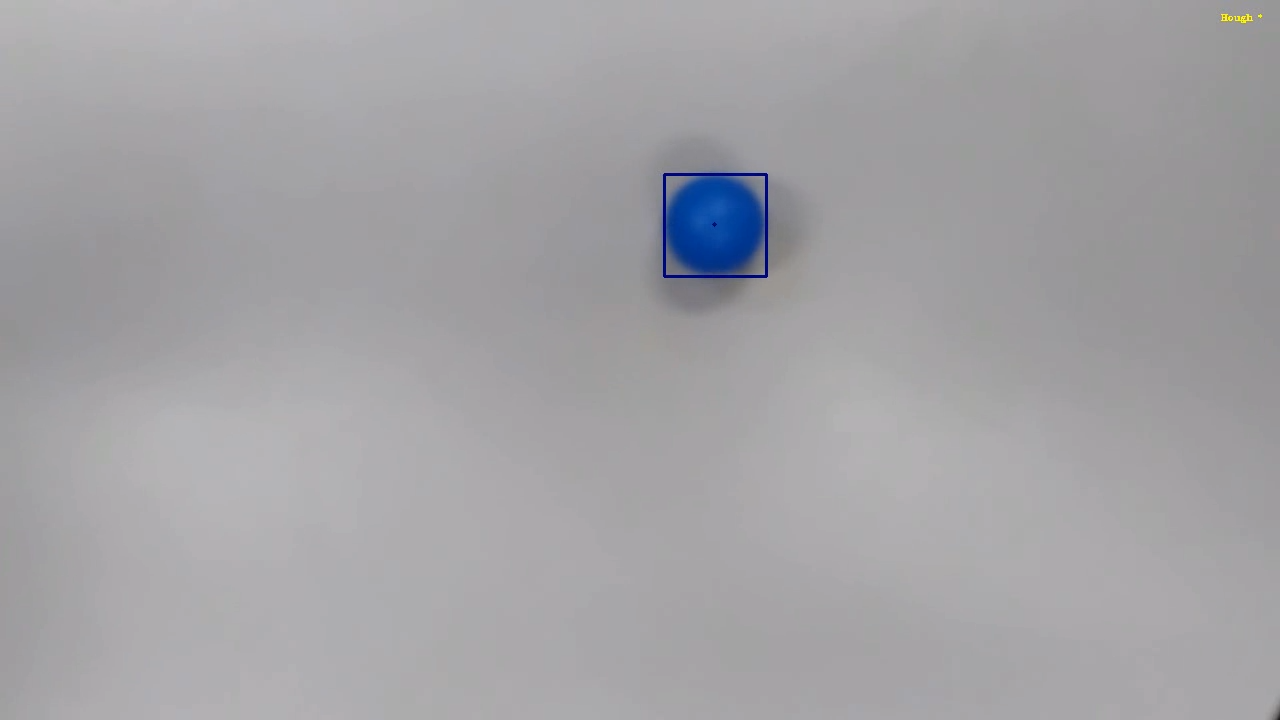
\includegraphics[scale=0.15]{images/single_color}}
\caption{Detection of a colored ball.}\label{fig:single_color}
\end{figure}

The color detection applied to every frame was able to track the ball
throughout the camera's view. This solution showed itself insufficient when
some objects were introduced, with different shapes other than of a sphere but
same color as the ball.

\bigbreak{}
\textbf{Two different color tracking:}
\bigbreak{}

The goal was to track each colored ball throughout the camera's view, not ever
mistaking one with another.

\begin{figure}[!h]
\centering
\setlength{\fboxsep}{1pt}
\setlength{\fboxrule}{1pt}
\fbox{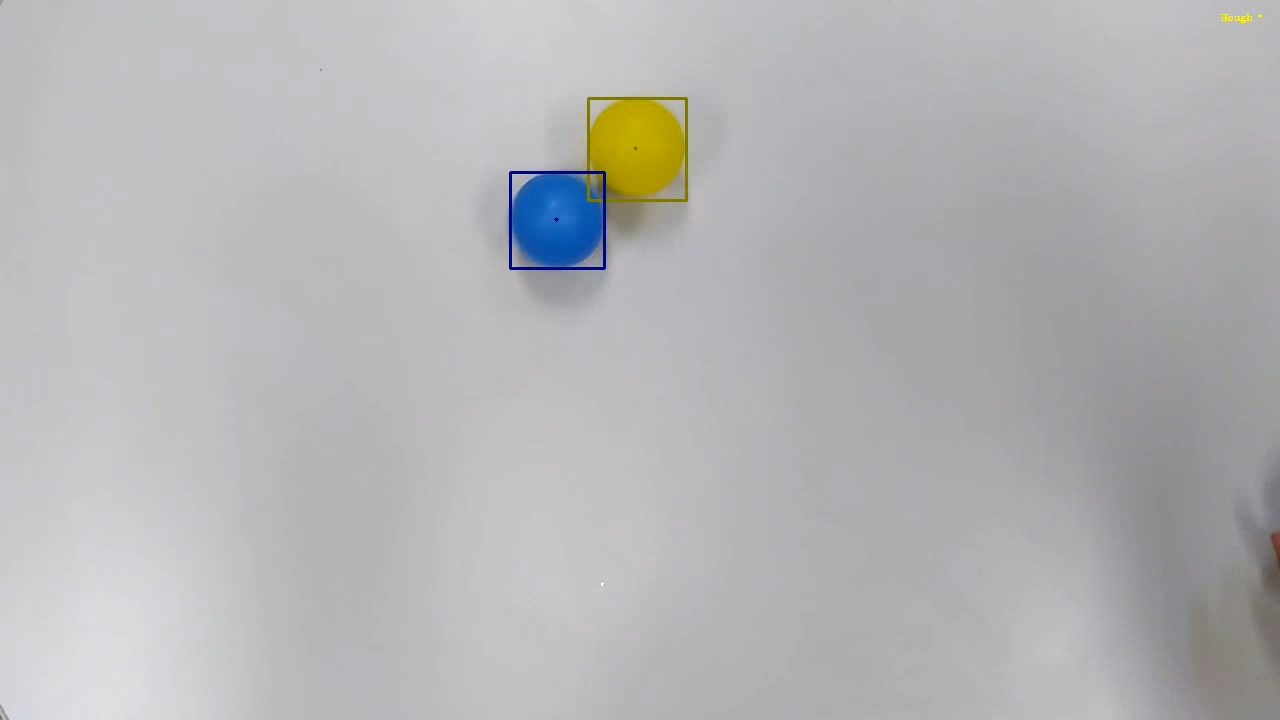
\includegraphics[scale=0.15]{images/diff_color}}
\caption{Detection of two balls with different colors.}\label{fig:diff_color}
\end{figure}

The fine tuning of the colors enabled the solution to isolate one ball from
the other, tracking them throughout the camera's view. This limits the
solution to be tuned at every application, indoor  and outdoor needs
distinct calibrations.

\bigbreak{}
\textbf{Two same color tracking:}
\bigbreak{}

The goal was to track each ball throughout the camera's view, not ever
mistaking one with another, now differentiating between two balls of the same
color.

\begin{figure}[!h]
\centering
\setlength{\fboxsep}{1pt}
\setlength{\fboxrule}{1pt}
\fbox{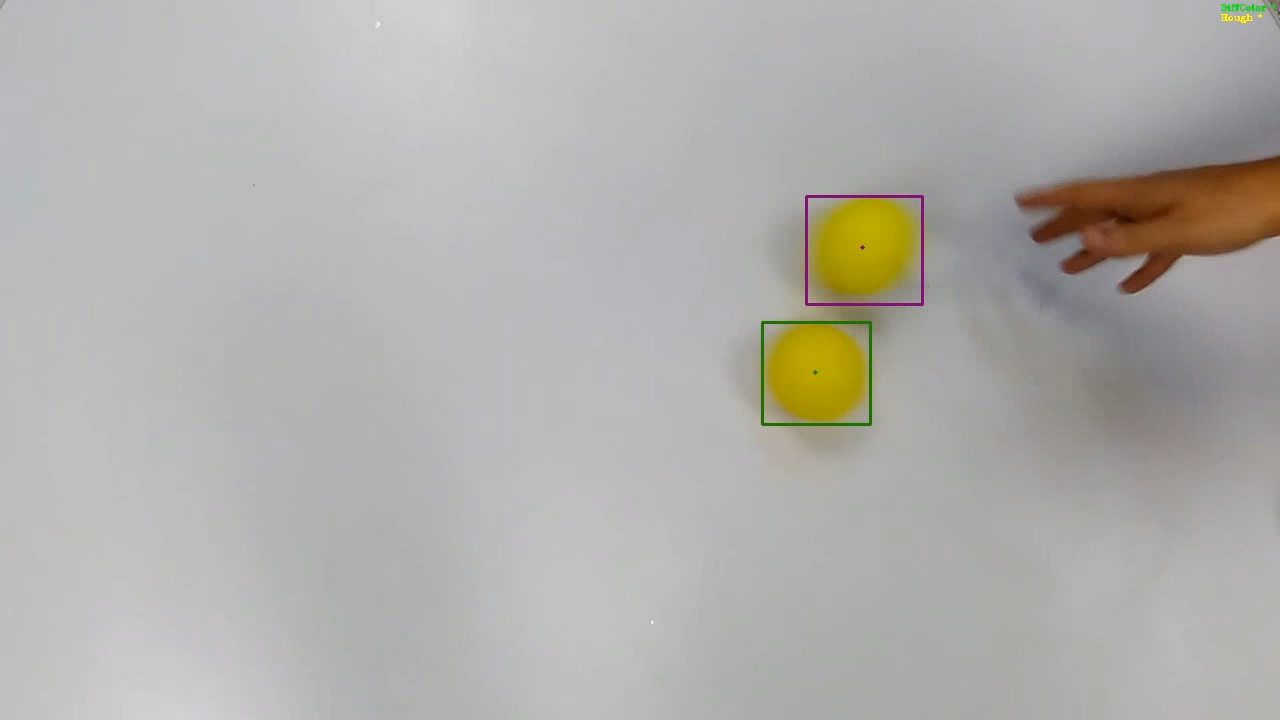
\includegraphics[scale=0.15]{images/same_color}}
\caption{Detection of two balls with the same color.}\label{fig:same_color}
\end{figure}

The size of the connected components regions found in the mask were used the
discriminate between the balls, the ratio between the first and second was
used and enabled the tracking to work, the solution is limited when the object
of interest moves away from the camera and becomes too small to pass the
threshold.

At this point the solution is able to detect and track the balls, it lacks the
ability to differentiate between $yellow\_ball\_1$ and $yellow\_ball\_2$, it
also mistakes other objects for balls and is quite expensive by detecting the
balls every frame.

\bigbreak{}
\textbf{Ball tracking alongside with other shapes:}
\bigbreak{}

The goal was to track a ball in a setup with many objects with different
shapes, but same color as the ball.

\begin{figure}[!h]
\centering
\setlength{\fboxsep}{1pt}
\setlength{\fboxrule}{1pt}
\fbox{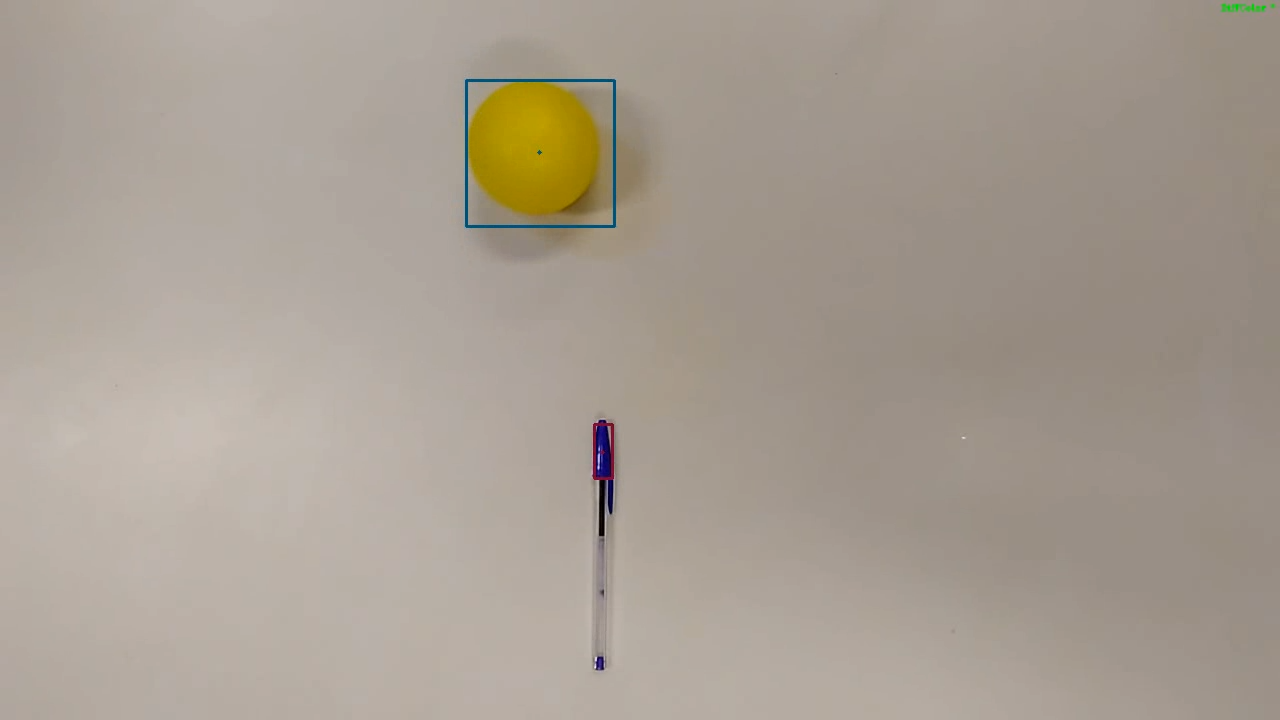
\includegraphics[scale=0.15]{images/not_hough}}
\caption{Detection before the Hough Circle Transform.}\label{fig:not_hough}
\end{figure}

As seen in Figure~\ref{fig:not_hough} the solution wasn't able to
differentiate the ball from the pen top. It happens because the shape of the
object has no weight in the detection process, so every object big enough and
in the color range of the chosen color will be detected as a ball. To solve
this we used the Hough Circle Transform.

\begin{figure}[!h]
\centering
\setlength{\fboxsep}{1pt}
\setlength{\fboxrule}{1pt}
\fbox{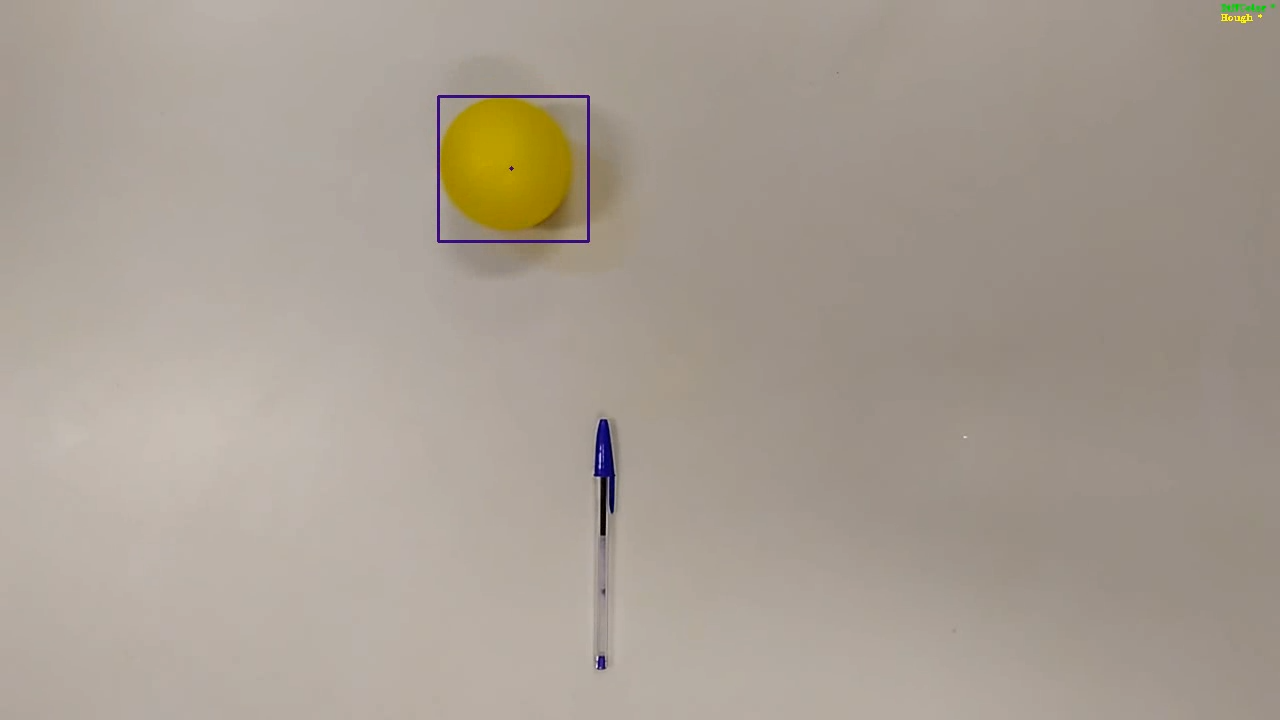
\includegraphics[scale=0.15]{images/yes_hough}}
\caption{Detection after the Hough Circle Transform.}\label{fig:yes_hough}
\end{figure}

In Figure~\ref{fig:yes_hough} using the Hough Circle Transform the solution
was able to ignore the pen top and track only the ball shaped object. This
solution is still limited by the time it took to adjust the parameters into
differentiate a pen top and a ball.

At this point the detection process is producing unambiguous results, but
since it happens at every frame it became too expensive to run in real time.

\bigbreak{}
\textbf{Motion flow tracking compared with color tracking:}
\bigbreak{}

The goal was to compare both solutions, Lucas Kanade motion flow tracking and
every frame color detection.

\begin{figure}[!h]
\centering
\setlength{\fboxsep}{1pt}
\setlength{\fboxrule}{1pt}
\fbox{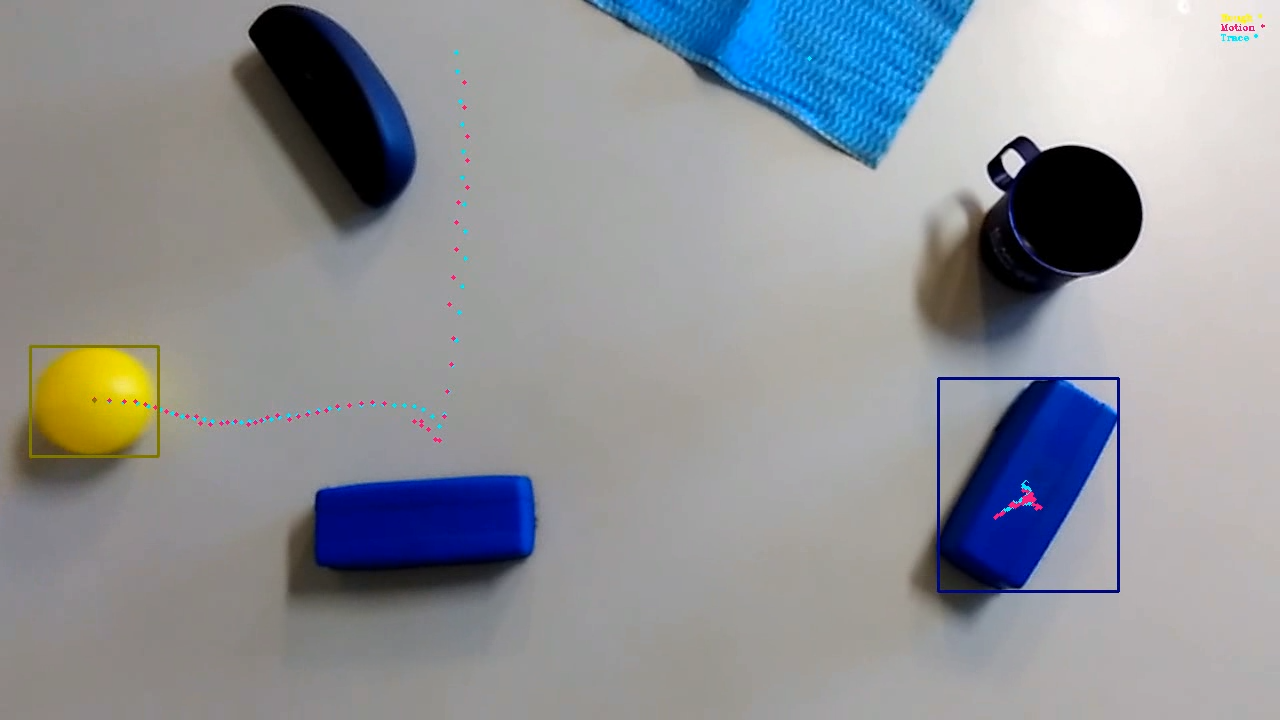
\includegraphics[scale=0.15]{images/motion_5}}
\caption{Lucas Kanade motion flow applied every 30 frames.}\label{fig:motion_30}
\end{figure}

Using the Lucas Kanade motion flow the solution would only apply the color
detection every $N$ frames and estimate the ball position in between
detection, this gap eliminated the need to detect it every frame enabling it
to perform in real time. The trade off is that the precision of the tracking
can diminish substantially depending on the gap size, and this experiment
showed that a gap of 30 frames was too large.

\begin{figure}[!h]
\centering
\setlength{\fboxsep}{1pt}
\setlength{\fboxrule}{1pt}
\fbox{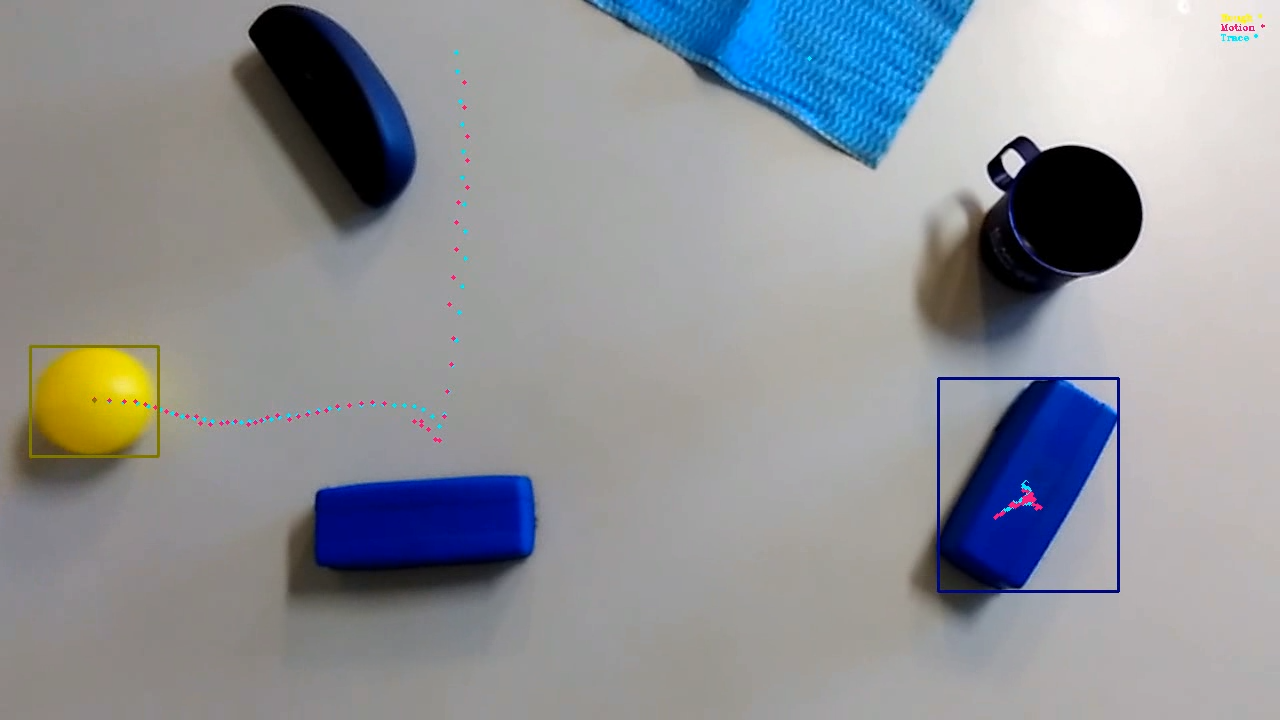
\includegraphics[scale=0.15]{images/motion_5}}
\caption{Lucas Kanade motion flow applied every 5 frames.}\label{fig:motion_5}
\end{figure}

Using a 5 frames gap the precision of the tracking was close to the color
tracking and the solution was still fast enough to operate in real time.
Although this solution couldn't keep tracking of the ball when it was occluded.

\bigbreak{}
\textbf{Occlusion tracking:}
\bigbreak{}

The goal was to compare the LK motion flow tracking and kalman filter
tracking, both applied towards an occlusion scenario.

\begin{figure}[!h]
\centering
\setlength{\fboxsep}{1pt}
\setlength{\fboxrule}{1pt}
\fbox{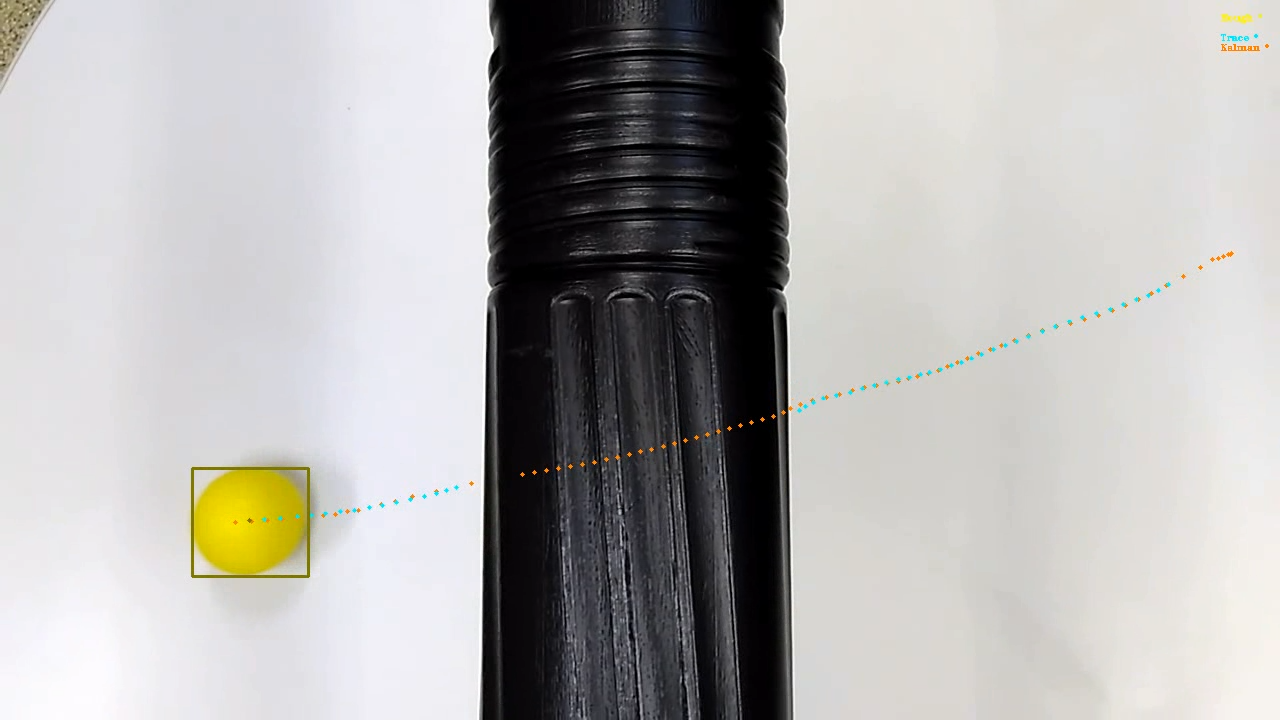
\includegraphics[scale=0.15]{images/occlusion}}
\caption{Kalman filter applied to overcome occlusion.}\label{fig:occlusion}
\end{figure}

The solution was able to overcome occlusion when the kalman filter was used in
such scenarios, since it was able to estimate the ball's trajectory. The
filter worked best with balls in low speed and couldn't estimate a position
if the ball changed directions whilst occluded.

\bigbreak{}
\textbf{Real world tracking:}
\bigbreak{}

The goal was to hard test all the features implemented in a real world
scenario to evaluate their precision.

\begin{figure}[!h]
\centering
\setlength{\fboxsep}{1pt}
\setlength{\fboxrule}{1pt}
\fbox{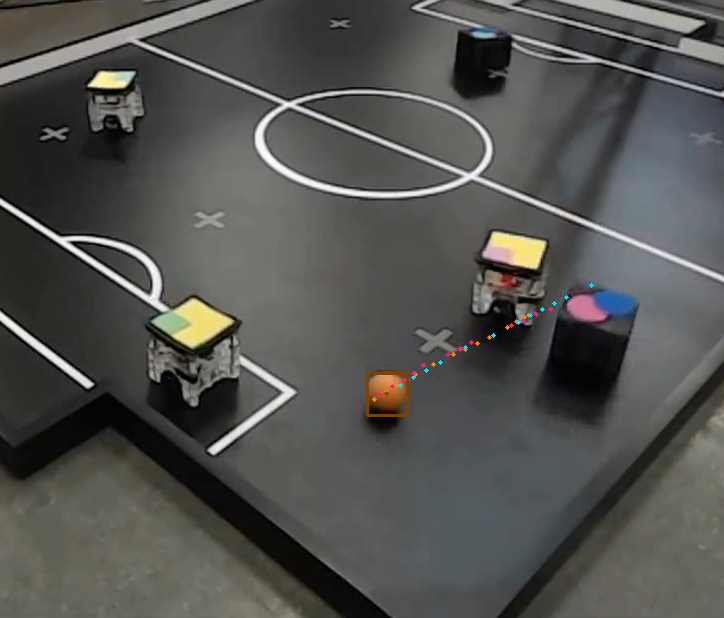
\includegraphics[scale=0.15]{images/robocup_1}}
\caption{All features applied in a Robocup soccer match.}\label{fig:robocup_1}
\end{figure}

When applied to a real world scenario the solution can keep tracking up to a
point, it fails whenever the ball drastically changes direction, specially
occluded, or when it moves too fast.

%-------------------------------------------------------------------------
\section{Conclusion}\label{sec:conclusion}

As seen the classic methods were able to track and overcome some of the
challenges presented in this project. It could even work good in a real example like the Robocup soccer match, however it is noticeable that the algorithm's precision is worse than in a totally controlled environment.

In harder scenarios, as a soccer, volleyball, and basketball games the algorithm had  bad results, in those scenarios physics models are used to describe the parabolic trajectory of the ball, or even  more complex models, which uses different clues, like the fact that a basketball player handling the ball o moves differently from the others.

In this project  many of the course's topics were covered and applied, clearing our sights towards their weakness and strength in each scenario. As future work, the color based detection could be replaced with a deep neural network in order to locate the initial position of the ball. This approach could improve the overall results, and enable the algorithm to deal with harder environments.

{\small
\bibliographystyle{ieee}
\bibliography{egbib}
}

\end{document}
